\documentclass[../main.tex]{subfiles} 
\begin{document}
\chapter{Low-Level softwarebeveiliging}
\section{Introductie}
Een \emph{implementation-level software vulnerability} is een fout in een programma die door een aanvaller kan worden misbruikt.
In dit hoofdstuk hebben we het concreet over \emph{memory corruption vulnerabilies}.
Deze zwakheden zijn enkel relevant voor onveilige talen.
Dat zijn programmeertalen die niet controleren of programma's het geheugen correct gebruiken.
Hieronder staat een voorbeeld in ANSI c in listing \ref{l:intro}. Omdat er nergens de lengte van de input argumenten wordt nagekeken kan men in geheugen schrijven waar dat niet zou mogen.
Op die manier kan er arbitraire code worden uitgevoerd (een \emph{code injection attack}).
 
\lstinputlisting[style=cstyle, label=l:intro]{\codeSrc/intro_example.c}

\subsection{Achtergrond informatie}
Er kan op verschillende manieren geheugen gealloceerd worden in C:
\begin{description}
	\item[Automatisch] via locale variablen in functies.	
	\item[Statisch] via globale variablen.	
	\item[Dynamisch] via \lstinline[style=cstyle]{void *malloc(size_t size);} en \lstinline[style=cstyle]{new}.
\end{description}
De programmeur is verantwoordelijk voor dit geheugenbeheer van het alloceren tot het de-alloceren.
Figuur \ref{f:mem_lay} geeft de \emph{process memory layout} weer van een programma.
Hierbij groeit de heap naar boven (hogere adressen) en de stack naar onder (lagere adressen).
Indien de voorbeeld code \ref{l:intro} wordt ge\"exploiteerd bevind de geinjecteerde code zich in de Stack.
\begin{figure}
\centering
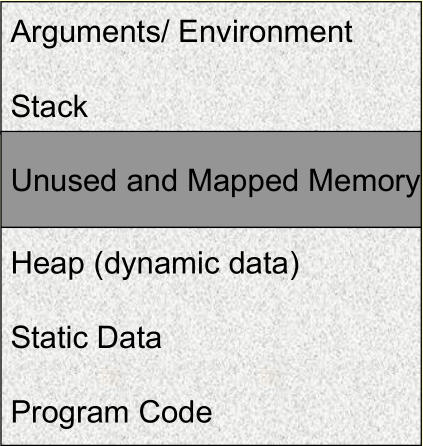
\includegraphics{\imageSrc/memory_layout.png}
\caption{Typische geheugen layout met bovenaan \textbf{hoge} adressen. De stack groeit van hoge naar lage adressen en de heap van lage naar hoge adressen.}
\label{f:mem_lay}
\end{figure}

Memory management in C is zeer fout-gevoelig typische bugs zijn o.a.:
\begin{itemize}
		\item Writing past the bound of array (zoals in listing \ref{l:intro})
		\item Dangling pointers (pointers die niet naar een geldig object wijzen.)
		\item Double freeing (Twee keer \lstinline[style=cstyle]{free()} aanroepen zodat nog gebruikt geheughen als ongebruikt wordt gemarkeert).
		\item Memory leaks (Stukken geheugen zijn niet correct vrijgegeven.)
\end{itemize}
Om effici\"entie redenen worden deze fouten in C niet at run time gededecteert.

Om onveilige code aan te vallen moet een aanvaller hetvolgende doen:
\begin{itemize}
		\item Een bug vinden die memory safety breekt.
				\begin{itemize}
						\item Buffer overflow
						\item Dereference van dangling pointer
						\item Gebruik van onveilige API functie. Die ofwel een buffer overflowt (e.g. \lstinline[style=cstyle]{strcpy()} ofwel intrinsiek onveilig geimplementeerd is in assembly (e.g. \lstinline[style=cstyle]{printf()}
				\end{itemize}
		\item Een interessante geheugen plaats vinden om te overschrijven.
				\begin{itemize}
								\item Code adressen/pointers: Return address, Function pointer in Virtual function table, Programma specifieke fuction pointers
								\item Pointers waar de aanvaller kan controleren wat er wordt geschreven als die dereferenced raakt (= Indirect pointer overwrite): redirect de pointer naar een andere interessante locatie en schrijf dan daar een zekere waarde.
				\end{itemize}
		\item Aanvals code in het geheugen van het process plaatsen.
\end{itemize}

\section{Aanvals voorbeelden}
\subsection{Stack-based buffer overflow}
De stack is een geheugen gebied dat wordt gebruikt om functie oproepen en returns at run time te beheren.
Per oproep wordt er een \emph{activation record} of \emph{stack frame} op de stack gepusht. Daarin zitten parameters, return address, lokale variablen, \ldots
Het is eenvoudig in te zien dat als er nu een lokale variable kan worden overflowt dat er interessante geheugen plaatsen ter beschikking komen.

In de onderstaande figuren leggen we een typisch Stack Based Buffer Overflow uit. Opgelet ook hier weer veronderstellen we dat bovenaan hoge addressen staan en dus overflowt een buffer naar boven.
In figuur \ref{f:stackBO1} tonen we een normale (niet aangevallen) stack waarbij het laatste stackframe dat van functie f0 is. De instructiepointer (IP) aan het begin van f0 staat en de (Saved) Frame Pointer ((S)FP) en Stack Pointer (SP) staan aangeduid.
\begin{figure}
\centering
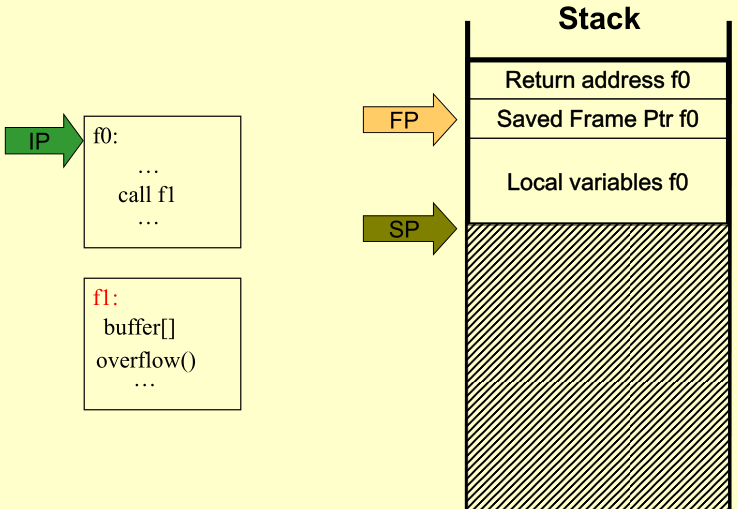
\includegraphics[scale=0.7]{\imageSrc/stackBO1.png}
\caption{Stack layout als de laatst opgeroepen functie f0 is.}
\label{f:stackBO1}
\end{figure}

Vervolgens in figuur \ref{f:stackBO2} wordt functie f1 opgeroepen. Een nieuw stackframe wordt op de stack gepusht. Let hierop dat in dit frame het return address nu wijst naar code net onder de call naar f1. De SFP wijst naar het frame van f0 en er daarachter plaats is voorzien voor de lokale variable \lstinline[style=cstyle]{buffer[]}. De stackpointer wijst natuurlijk net voorbij het frame van f1.
\begin{figure}
\centering
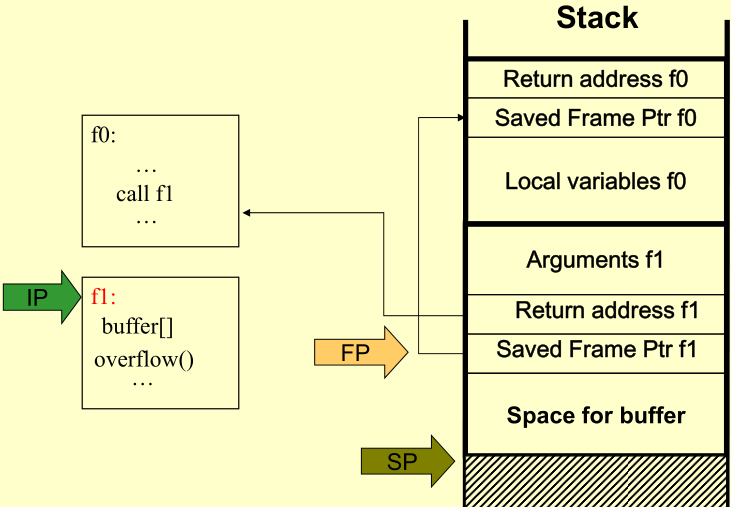
\includegraphics[scale=0.7]{\imageSrc/stackBO2.png}
\caption{Stack layout na call van functie f1.}
\label{f:stackBO1}
\end{figure}

In deze figuur wordt de overflow aangeduid. Als er geen bounds check gebeurdt kan de buffer blijven groeien en zo eerst de SFP, en dan het return address overschrijven. Door nu in het buffer uitvoerbarde code te steken en het return address naar die code te doen verwijzen kan er alles met het programma worden gedaan.
\begin{figure}
\centering
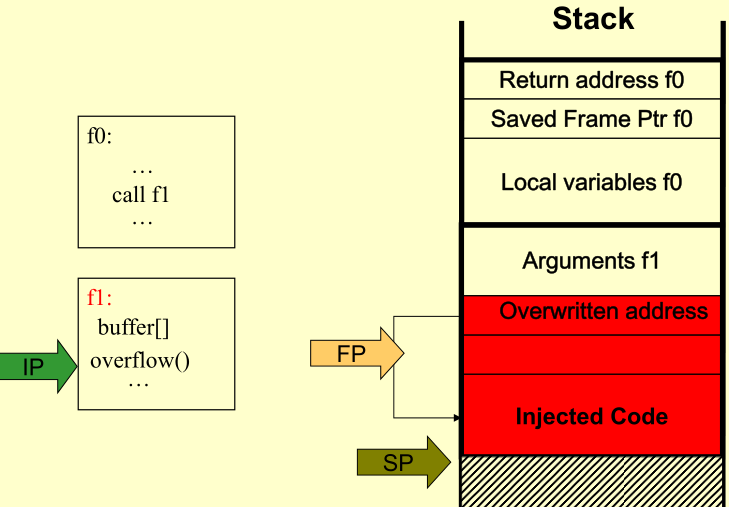
\includegraphics[scale=0.7]{\imageSrc/stackBO3.png}
\caption{Stack layout na buffer overflow attack op de lokale variable buffer in functie f1.}
\label{f:stackBO3}
\end{figure}
Het voorbeeld dat we in de introductie zagen (zie listing \ref{l:intro}) is een goed voorbeeld van een programma kwetsbaar voor een buffer overflow attack.

Code die vaak wordt gebruikt om te injecteren is het starten van een nieuwe shell. Om dit te doen wordt er zogenaamde shellcode gebruikt. Dit is een string van hexadecimale codes die dan worden geinterpreteerd als programma code. Hieronder vind u een voorbeeld die op Linux systemen met een intel x86 architectuur kan gebruikt worden om de sh shell te starten.

\begin{blockquote}
		durr
	%"xeb\x1f\x5e\x89\x76\x08\x31\xc0\x88\x46\x07\x89\x46\x0c\xb0\x0b\x89\xf3\x8d\x4e\x08\x8d\x56\x0c\xcd\x80\x31\xdb\x89\xd8\x40\xcd\x80\xe8\xdc\xff\xff\xff/bin/sh"
\end{blockquote}

Om een stack based buffer overflow werkend te krijgen zijn er heel veel details waar de aanvaller rekening mee moet houden: O.a. 

\subsection{Heap-based buffer overflow}

\subsection{Return-to-libc attacks}
\subsection{Data-only attacks}
\section{Verdedigings voorbeelden}
\subsection{Stack canaries}
\subsection{Non-executable data}
\subsection{Control-flow integrity}
\subsection{Layout randomization}
\section{Conclusie}
\end{document}
